\documentclass[a4paper]{report}

\usepackage{../mathstemplate}

\date{IV семестр, весна 2024 г.}
\title{Дифференицальная геометрия. Неофициальный конспект}
\author{Лектор: Нина Дмитриевна Лебедева \\ Конспектировал Леонид Данилевич}

\begin{document}
    \shorthandoff{"}
    \maketitle
    \tableofcontents
    \newpage
    \setcounter{lection}{0}


    \chapter{Риманова геометрия}
    \newlection{14 февраля 2024 г.}
\section{Гладкие многообразия}
    \definition[Топологическое многообразие]{
        Хаусдорфово топологическое пространство $M$ со счётной базой, такое что $\forall x \in M: \exists U \ni x: U \sim \R^n$.
        Данное число $n$ называется \emph{размерностью} многообразия, пишут $\dim M = n$, или часто пишут это число верхним индексом: $M^n$.
    }
    Далее пусть $M^n$ --- топологическое многообразие.
    \definition[Карта]{
        Пара из открытого $U \subset M^n$, и гомеоморфизма $\phi: U \map \Omega$, где открытое $\Omega \subset \R^n$.
    $U$ называется \emph{носителем карты}.
    }
    <<В половине случаев в литературе картой называется обратное отображение>>.
    \definition[Атлас]{
    Набор карт $(U_i, \phi_i)$, таких, что $\bigcup\limits_{i}U_i = M$.
    }
    Пусть даны две карты $(U, \phi)$ и $(V, \psi)$.
    Далее удобно считать, что их носители пересекаются: $U \cap V \ne \o$, иначе определение не несёт смысла.
    \definition[Отображение перехода]{
    Отображение $\psi \circ \phi^{-1}: \phi(U \cap V) \map \psi(U \cap V)$.
    }
    \definition[Карты $(U, \phi)$ и $(V, \psi)$ согласованы]{
        Отображение перехода и ему обратное гладкие.
    }
    \definition[Гладкий атлас]{
    Атлас, такой, что любые две карты согласованы.
    }
    Далее все атласы предполагаются гладкими.
    \definition[Атласы эквивалентны]{
        Их объединение (то есть все карты из первого и из второго атласа вместе взятые) --- тоже гладкий атлас.
    }
    \proposal{
    Эквивалентность атласов --- отношение эквивалентности.
    }
    \definition[Гладкая структура на многообразии]{
    Максимальный гладкий атлас (атлас, к которому нельзя добавить карт).
    }
    \note{
        К атласу можно добавить произвольное количество карт, согласованных с теми, что в атласе, и они будут согласованы между собой.
    В частности, для задания гладкой структуры достаточно произвольного атласа $A$: в $A$ можно добавить всевозможные карты, согласованные с картами из $A$, и он станет максимальным.
    }
    \definition[Гладкое многообразие]{
    Многообразие с гладкой структурой.
    }
    \examples[Атласы]{
    \item Стандартная гладкая структура на $\R^n$ задаётся атласом $\{(\R^n, \id)\}$.
        \item В частности, стандартная структура на $\R^1$ задаётся атласом $\{(\R^1, [x \mapsto x])\}$.
    \item Можно задать нестандартную структуру на $\R^1$: $\{(\R^1, [x \mapsto x^3])\}$.
    \precaution{
        Это действительно гладкая структура, хотя обратное отображение ${[x \mapsto x^{\nicefrac{1}{3}}]}$ не гладкое.
        Тем не менее, определение и не требует гладкости от него.
    }
    \item Пусть $f = \all{x, & x \ge 0 \\ \frac{1}{2}x,&x \le 0}$. Тогда $\{(\R^1, f)\}$ --- тоже гладкий атлас на $\R^1$.

    Тем не менее, любые два атласа из приведённых выше атласов на $\R^1$ не эквивалентны --- отображения перехода получаются не гладкими.
    \item Гладкая структура на сфере задаётся двумя картами: пусть $S^2$ --- сфера с северным полюсом $N$ и южным $S$, пусть $f, g$ --- стереографические проекции с данными полюсами.
        Тогда ${\{(S^2 \sm \{N\}, f), (S^2 \sm \{S\}, g)\}}$ --- атлас.
    }
    \note{
    Если $M$ --- гладкое многообразие, и открытое $W \subset M$, то на $W$ естественным образом определена гладкая структура, наследующаяся с $M$.
    }
    \subsection{Гладкие отображения}

    Пусть $M^m, N^n$ --- гладкие многообразия, $A_M, A_N$ --- соответствующие атласы.
    Рассмотрим отображение $f: M \map N$.
    \definition[Координатное представление $f$ в картах $(U, \phi)$ на $M$ и $(V, \psi)$ на $N$]{
        Такое $\tilde{f}: \phi(U) \map \psi(V)$, что диаграмма коммутативна везде, где определена (то есть $\tilde{f} = \psi \circ f \circ \phi^{-1}$ на $\phi(U \cap f^{-1}(V))$).
        % https://q.uiver.app/#q=WzAsNCxbMCwxLCJcXHBoaShVKSJdLFsxLDEsIlxccHNpKFYpIl0sWzAsMCwiVSJdLFsxLDAsIlYiXSxbMiwwLCJcXHBoaSJdLFszLDEsIlxccHNpIl0sWzIsMywiZiJdLFswLDEsIlxcdGlsZGV7Zn0iXV0=
        \[\begin{tikzcd}[ampersand replacement=\&]
              U \& V \\
              {\phi(U)} \& {\psi(V)}
              \arrow["\phi", from=1-1, to=2-1]
              \arrow["\psi", from=1-2, to=2-2]
              \arrow["f", from=1-1, to=1-2]
              \arrow["{\tilde{f}}", from=2-1, to=2-2]
        \end{tikzcd}\]
    }
    Далее считаем, что $f: M \map N$ непрерывна (эквивалентно, все координатные представления непрерывны).
    \definition[$f$ гладкое]{
    Любое координатное представление --- гладкое.
    }
    \definition[$f$ --- гладкое в точке $x \in M$]{
    Найдётся окрестность $U_x \ni x$ и карты $(U, \phi)$, $(V, \psi)$ (где $V \ni y \coloneqq f(x)$), такие, что $U_x \subset U$ и сужение на $U_x$ координатного представления $f$ --- гладко.
    }
    \properties[Гладкие отображения]{
    \item Гладкость в точке не зависит от выбора карт.
    \item Гладкость отображения не зависит от выбора атласа в одном классе эквивалентности.
    \item Отображение гладкое $\iff$ оно гладкое в любой точке. \comment{На лекции было доказательство $\when$.}
    \item Пусть $f: M \map N, g: N \map K$ гладкие. Тогда их композиция $g \circ f$ гладкая.
    \item Тождественное отображение гладкое, если в образе и прообразе выбраны эквивалентные атласы.
    \item Определение гладкости отображения совпадает с определением гладкости из матанализа (если считать, что $M \subset \R^n$ открыто, и порождающий атлас состоит из тождественной карты)
    }
    \definition[Диффеоморфизм $f: M \map N$]{
    Гладкое $f$, такое, что $f^{-1}$ --- тоже гладкое.
    }
    \definition[Многообразия $M$ и $N$ диффеоморфны]{
    Между ними существует диффеоморфизм.
    }
    Понятно, что диффеоморфность --- отношение эквивалентности.
    \statement{
    Если $M^m \overset{\text{диф}}\sim N^n$, то $m = n$.
    \provehere{
    Рассмотрим произвольную $x \in M$.
    Пусть $f: M \map N$ --- диффеоморфизм, пусть $\tilde{f}$ --- его координатное представление.
        Тогда $\tilde{f}^{-1}$ --- координатное представление $f^{-1}$, откуда $\tilde{f}^{-1}$ --- тоже гладкое.
     Рассмотрим дифференциал $\d_{\tilde{f}}(x, \_)$, это изоморфизм векторных пространств, значит, $m = n$.
    }
    }
    По умолчанию всегда считается, что на $\R^m$ введена стандартная гладкая структура.
    \proposal{
        Пусть $M$ --- гладкое многообразие, тогда карта --- диффеоморфизм между $U$ и $\phi(U)$.
        Обратно, любой диффеоморфизм между открытым подмножеством $W \subset M$ и областью $\Omega \subset \R^m$ --- карта.
        \provehere{
            \[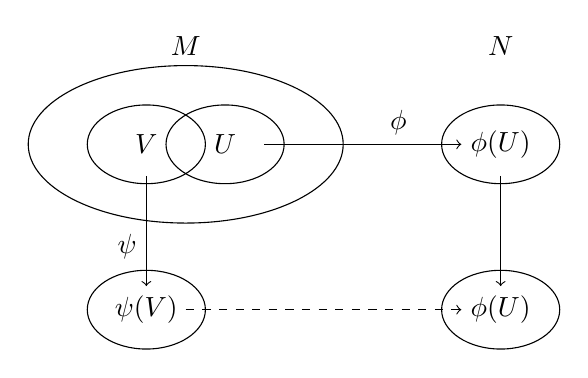
\begin{tikzpicture}
                  \draw (-2,2) ellipse (2cm and 1cm);
                  \draw (-2.5,2) ellipse (0.75cm and 0.5cm);
                  \draw (-1.5,2) ellipse (0.75cm and 0.5cm);
                  \node at (-2.5,2) {$V$};
                  \node at (-1.5,2) {$U$};
                  \node[above] at (-2,3) {$M$};
                  \draw[->] (-1, 2) -- (1.5,2);
                  \node[above] at (0.7,2) {$\phi$};
                  \draw (2,2) ellipse (0.75cm and 0.5cm);
                  \node at (2,2) {$\phi(U)$};
                  \node[above] at (2,3) {$N$};
                  \draw[->] (2,1.6) -- (2,0.2);
                  \node[right] at (2,1) {$\id$};
                  \draw (2,-0.1) ellipse (0.75 cm and 0.5 cm) node {$\phi(U)$};
                  \draw[->] (-2.5,1.6) -- (-2.5,0.2);
                  \node[left] at (-2.5, 0.7) {$\psi$};
                  \draw (-2.5,-0.1) ellipse (0.75 cm and 0.5 cm) node {$\psi(V)$};
                  \draw[->,dashed] (-2,-0.1) -- (1.5,-0.1);
            \end{tikzpicture}\]
            Гладкость карты, как диффеоморфизма, эквивалентна тому, что карта согласована с остальными в атласе: пунктирная стрелка $\psi(U \cap V) \map \phi(U \cap V)$ одновременно является отображением перехода между картами $(U, \phi)$ и $(V, \psi)$, и координатным представлением $\phi$ в картах $(V, \psi), (U, \id)$.
        }
    }
    \corollary{Диффеоморфизм $f: M \map N$ задаёт естественную биекцию между картами $M$ и картами $N$ (а ещё между (максимальными) атласами $M$ и (максимальными) атласами $N$). }
\end{document}
